\chapter{Implementation}
This chapter describes the implementation of the CloudASR platform.
The platform provides API for both batch and online speech recognition mode
  and it has an annotation interface for adding transcriptions to submitted recordings.
The implementation was also affected by the following requirements:

\begin{itemize}
  \item
    \textbf{Scalability} -
      because the speech recognition is a demanding process in terms of computational resources,
        it is not possible to handle many parallel requests on one machine.
      Therefore the CloudASR architecture had to be designed to be able to scale across many machines.

  \item
    \textbf{Easy deployment} -
      complex systems as CloudASR is have many dependencies and a difficult deployment process,
        which makes their maintenance hard.
      CloudASR should have as few dependencies as possible and only one command deployment.

  \item
    \textbf{Customizability} -
       there are already several web services that provide an API for speech recognition,
         but they are not easily customizable.
       Thus, the second requirement was to be able to host any Kaldi model on  the CloudASR platform.
       Moreover, the CloudASR platform should be able to run any ASR system,
         if the users implement a wrapper for that system.

\end{itemize}


\section{Architecture}
In order to meet the aforementioned scalability requirement
  the platform had to be designed from the very beginning to be able to run on many machines.
As a result, the architecture consists of several nodes
  that communicate with each other by sending messages over ZeroMQ sockets
  (each node acts as an actor as described in \cite{hewitt1977viewing}).

The architecture was also affected by the fact
  that it is not possible to start an ASR system when the user sends a request,
  because the ASR systems need some time to load decoding graphs in the memory,
  which would add some unnecessary latency.
To solve this problem the platform uses Master-Worker architecture,
  which also makes it possible to handle requests for various languages at the same time.

The CloudASR architecture as described in Figure~\ref{fig:architecture} consists of several types of nodes that can run on different machines.
These nodes are \textbf{Master}, \textbf{Worker}, \textbf{API}, \textbf{Web},  and \textbf{Recordings Saver}.
In the following section each node will be described in detail.


\begin{figure}[h]
  \centering
  \includegraphics[width=0.75\textwidth]{./img/architecture.pdf}

  \caption{
    An overview of the CloudASR architecture.
    The most important node is \textbf{Master} to which \textbf{Workers} send heartbeats with their state.
    The client requests are handled by \textbf{API} which communicates with Master and Workers.
    The processed recordings are sent to \textbf{Saver} which saves them and serves them via HTTP.
    An annotation interface and an online demo are hosted by \textbf{Web}.
    Finally, there are also two external nodes: \textbf{HAProxy}
      which load-balances requests between particular application instances
      and \textbf{DB} which stores information about processed recordings.
  }
  \label{fig:architecture}
\end{figure}


\subsection{Master}
The main task of Master is to keep track about running workers and to schedule tasks to them.
In order to be able to handle requests for various languages
  Master monitors state of each worker
  and it has a queue of waiting workers for each language,
    so that when API asks for a worker Master can return an address of an available worker.

The workers can be in four different states:
  \textbf{started}, \textbf{waiting}, \textbf{working} and \textbf{not responding}
  and they send four different heartbeats, small messages with an information about their state, to Master:
  \textbf{started}, \textbf{waiting}, \textbf{working} and \textbf{finished}.

The life cycle of the worker as described in Figure~\ref{fig:worker-state} starts in the \textbf{started} state,
  after that it moves to the \textbf{waiting} state by sending the \textbf{waiting} heartbeat.
The worker remains in the waiting state until \textbf{Master assigns a tasks} to it,
  then it moves to the \textbf{working} state
  where it remains as long as it is working.
In the working state worker sends working heartbeats periodically,
  to inform Master that it is working and it did not fail.
At the end of the task the Worker sends \textbf{finished} heartbeat
  and Master changes the state of the Worker to the \textbf{waiting} state.

Additionally, when a worker crashes during the processing of the task and it gets restarted,
  it sends started heartbeat again,
  which informs Master, that the worker was restarted and it adds it to the queue again.
When a worker does not send any heartbeat for 10 seconds,
  the master sets the worker state to \textbf{not responding}.
But as soon as the worker sends any heartbeat,
  the master will set the worker to the appropriate state.

\begin{figure}[h]
  \centering
  \includegraphics[width=0.75\textwidth]{./img/worker-state.pdf}

  \caption{
    The life cycle of the worker starts in in the \textbf{started} state,
      after that it moves to the \textbf{waiting} state by sending the \textbf{waiting} heartbeat.
    The worker remains in the waiting state until \textbf{Master assigns a tasks} to it,
      then it moves to the \textbf{working} state
      where it remains as long as it is working.
    In the working state worker sends working heartbeats periodically,
      to inform Master that it is working and it did not fail.
    At the end of the task the Worker sends \textbf{finished} heartbeat
      and Master changes the state of the Worker to the \textbf{waiting} state.
  }
  \label{fig:worker-state}
\end{figure}

Unfortunately, Master is a single point of failure of the CloudASR platform.
When Master stops working no speech recognition requests can be processed,
  because the API containers will not know to which worker they can forward the request.
But as soon as Master starts working the platform should be available again.


\subsection{Worker}
Worker acts as a wrapper for an ASR system.
By default Pykaldi is used but any other ASR system can be used
  if the user implements a python wrapper for that system.
Because CloudASR should be able to process very long recordings in the online speech recognition mode,
  it is necessary to split the recordings into smaller chunks
  that can be processed with limited computational resources.
For that purpose VAD component from Alex Statistical Dialogue Systems Framework \cite{jurcicek2014alex} is used to detect silence in a speech,
  because the speech can be split at that point without any large negative effect on the accuracy of the transcriptions.


\subsection{API}
The main task of API is to forward requests from the clients to the workers.
When API receives a request from a client,
  it sends a message to Master with a request for a worker address for the given language.
If there is any available worker, Master returns its address,
  otherwise Master returns an error which is forwarded back to the client.
Then API sends the submitted recording to the worker,
  which processes it
    and sends back either interim results for the online speech recognition mode
      or final results for the batch speech recognition mode.
Finally, API sends a response with the results to the client.

The API is built on top of Flask framework with enabled asynchronous processing
  which allows single API container to process many parallel requests,
  because there are no blocking operations in the API container -
  it just receives requests from clients and forwards them via ZeroMQ to the workers.



\subsection{Web}
CloudASR platform has a web interface with an online demo and an annotation interface.
The online demo (See Figure~\ref{fig:webdemo}) allows users to try out CloudASR directly in their web browsers.
It has two modes, namely, dictation mode, which only shows the best transcription of the recording,
  and evaluation mode, which also allows users to confirm that the transcription of the recording is correct.

\begin{figure}[h]
  \centering
  \includegraphics[width=0.95\textwidth]{./img/demo.pdf}

  \caption{Screen of the Web Demo}
  \label{fig:webdemo}
\end{figure}

Even though the annotation interface allows anonymous users to add transcriptions to recordings,
  the users are encouraged to log in via their Google Account,
  because then it is possible to track their transcriptions
    and make useful insights about the quality of their transcriptions.

The annotation interface distinguishes between two types of user roles: users and administrators.
Normal users are only allowed to add transcriptions (See Figure~\ref{fig:annotation-interface}) to the recordings selected by CloudASR,
  but administrators can view every recording with its transcriptions.

In order to get the most of the normal user transcriptions,
  a recording, which should be transcribed by the user,
  is selected randomly from all recordings for the given language with confidence lower than 0.8,
    because it is not necessary to transcribe recordings with correct transcriptions.
This allows to collect transcriptions for all recordings uniformly
  and then it is up to the administrator to decide which transcription is the best.

\begin{figure}[h]
  \centering
  \includegraphics[width=0.95\textwidth]{./img/annotation.pdf}

  \caption{Screen of the Annotation Interface}
  \label{fig:annotation-interface}
\end{figure}



\subsection{Recordings saver}
The main task of the Recordings saver is to save and serve recordings processed by workers.
When the worker finishes recognition
  it sends the recording with its n-best hypotheses to the Recording saver via ZeroMQ socket.
The saver saves the wave file to the file system
  and it saves the n-best hypotheses to the database so that they can be used in the future.


\section{Scalability}
As mentioned before, one of the key requirements for the CloudASR platform was scalability.
To successfully fulfill this requirement architecture was split into smaller nodes,
  which communicate with each other by sending messages over ZeroMQ sockets.
This enables the platform to run on several machines.
Additionally, the heartbeating makes it possible to scale workers dynamically without need to stop the platform.
Finally, load-balancing allows to run several API nodes and spread the load between.
Yet, this solution is limited by the network capacity,
  but it is possible to deploy the CloudASR to a different data center
  and load balance between data centers.
This makes the CloudASR platform almost infinitely scalable.


\section{Deployment}
The CloudASR platform supports two types of deployment: single host and multi host.
Single host deployment allows users to run CloudASR directly on their machines with just one dependency installed - Docker.
Whereas multi host deployment allows users to run CloudASR on a set of machines with Mesos installed.

Users can specify which workers they want to run in a configuration file,
  see Figure~\ref{fig:cloudasr-json} for an example.
In this file they can specify names of Docker images for the workers,
  number of instances of these workers
  and a model name with which the worker will be available for speech recognition.
Also, users have to specify runtime variables such as IP address of a slave where the Master should run,
  MySQL connection string and
  a domain name that HAProxy will use to route requests to the running platform.
Finally, users have to specify credentials for Marathon if they want to run the platform on a Mesos cluster.
After that they can run CloudASR locally with \texttt{make run\_locally} command
  or on a Mesos Cluster with \texttt{make run\_on\_mesos} command.

\begin{figure}[h]
  \verbatiminput{snippets/cloudasr.json}

  \caption{
     An example of the CloudASR configuration \texttt{deployment/cloudasr.json}
       that specifies how to run 5 cs-alex workers and 5 en-towninfo workers
       using respective Docker image.
     With this configuration file the CloudASR platform can be run locally with command \texttt{make run\_locally}
       or on a Mesos cluster with command \texttt{make run\_on\_mesos}.
  }
  \label{fig:cloudasr-json}
\end{figure}


In order to ensure quality and stability of the CloudASR platform,
  two practises were used during the development:
  \textbf{Continuous Integration} \cite{fowler2006continuous} and \textbf{Continuous Delivery} \cite{humble2010continuous}.
The goal of these practises is to build, test and deploy the CloudASR platform as often as possible,
  to get feedback from the real usage.
To achieve that the CloudASR platform uses Jenkins-CI server
  that watches the CloudASR git repository
  and on every push to the repository it builds Docker images,
  tests the code
  and pushes the built Docker images to the Docker Registry.
After that it is possible to deploy the CloudASR platform with a specific version
  and it is also possible to switch back to the older versions when anything goes wrong.
To minimize failures CloudASR is deployed first to the development environment,
  where the users can test it
  and then it can be deployed to the production environment.


To ensure stability of CloudASR all crucial parts of the platform are covered with tests,
  namely unit tests, integration tests and end-to-end tests.

Each node was implemented with two main design patterns in mind, namely Dependency Injection \cite{fowler2004inversion} and Factory Method \cite{gamma1993design}.
Usage of these patterns together with message oriented architecture made it possible to unit test the whole platform easily,
  because it enabled to pass test doubles into the nodes
  and then send fake messages needed to test a correct behaviour of the node.
A typical unit test structure of the CloudASR platform node looks like a test in Figure~\ref{fig:unit-test}.

In addition to unit tests there are also integration tests,
  which test the factory methods that create production ready nodes,
  and end-to-end tests,
  which test that both batch and online recognition mode requests are handled correctly.
This test suite ensures that developers do not break anything
  and it also gives them confidence to change the code without fear.

\begin{figure}[h]
  \verbatiminput{snippets/unit_test.py}

  \caption{An example of unit test that tests communication between nodes.}
  \label{fig:unit-test}
\end{figure}


\section{Customizability}
The second requirement for CloudASR is customizability in terms of acoustic and language models.
The platform supports creating new workers with various acoustic and language models and
  it also supports creating new workers with arbitrary ASR systems.
An overview on the customization process is described in the following section.


\subsection{Worker with New Kaldi Models}
In order to create a new worker with new Kaldi models a worker Docker image has to be made.
The image is created in several steps.
First, users have to create a script \texttt{download\_models.sh}
  that will download all necessary files from their server,
  see Figure~\ref{fig:download-models} for example.
Second, they have to create a configuration file \texttt{config.py} with an appropriate configuration for the downloaded models,
  see Figure~\ref{fig:config-py}.
Finally, they have to copy a Dockerfile (see Figure~\ref{fig:worker-dockerfile}for example) for the worker
  and build the docker image with the appropriate command.
After that users can use the new worker in their application in the similar way as they use other models.

\begin{figure}[h]
  \verbatiminput{snippets/download_models.sh}

  \caption{An example of download\_models.sh script.}
  \label{fig:download-models}
\end{figure}

\begin{figure}[h]
  \verbatiminput{snippets/config.py}

  \caption{An example of config.py script.}
  \label{fig:config-py}
\end{figure}

\begin{figure}[h]
  \verbatiminput{snippets/Dockerfile_cs_alex}

  \caption{An example of worker Dockerfile.}
  \label{fig:worker-dockerfile}
\end{figure}


\subsection{Worker with Arbitrary ASR System}
Even though CloudASR supports only Kaldi out of the box, other ASR systems can be used too.
Again, the only thing that the users have to do is to create a worker docker image with their ASR system.
The only step that differs from the previous process is
  that the users have to implement and add to the Dockerfile a script \texttt{asr.py} with their own \texttt{create\_asr} method
  that returns \texttt{ASR} class with these methods:

\begin{itemize}
  \item
    \texttt{reset()} - this method is called after every request
      and it can be used to reset the underlying ASR system.

  \item
    \texttt{recognize\_chunk(pcm)} - this method is used to process small chunks of recordings.
      The method should accept pcm chunks with frame rate 16000
        and it should return an interim hypothesis in the form of a tuple \texttt{(confidence, transcript)}.

  \item
    \texttt{get\_final\_hypothesis} - this method is called at the end of every request,
      it should return a list of n-best hypotheses in the form of a tuple \texttt{(confidence, transcript)}.

\end{itemize}

The creation of such a script is illustrated in Figure~\ref{fig:dummyasr} on the DummyASR class,
  which will also be used for benchmark purposes in the Chapter~\ref{chapter:evaluation}.

\begin{figure}[h]
  \verbatiminput{snippets/dummy_asr.py}

  \caption{An example of alternative ASR implementation.}
  \label{fig:dummyasr}
\end{figure}


It is important to note that the new worker Docker images will be available only on the machine
  where they were built.
If the users want to use these workers on multiple machines, they have to push them to their docker registry
  or they can update Jenkins scripts \texttt{build\_workers.sh} and \texttt{push\_workers.sh}
  and Jenkins will do that for them.


\section{Example of API Usage}
The CloudASR platform supports both batch and online speech recognition.
In the batch mode users send wave files to the API using HTTP POST request
  and they receive a json with n-best transcriptions.
Users can specify which worker they want to use in \texttt{lang} parameter.
The batch mode has a similar interface to Google Speech API,
  which enables users to switch to CloudASR seamlessly.
An example of batch recognition API usage is illustrated on a simple curl command in Figure~\ref{fig:curl}
  and a response from the API is shown in Figure~\ref{fig:curl-response}.

\begin{figure}[h]
  \verbatiminput{snippets/curl.bash}

  \caption{An example of batch speech recognition mode request for an en-towninfo worker using curl.}
  \label{fig:curl}
\end{figure}

\begin{figure}[h]
  \verbatiminput{snippets/curl.json}

  \caption{An example of batch recognition mode response.}
  \label{fig:curl-response}
\end{figure}

In contrast to batch mode in online mode users send PCM chunks of a recording while the recording is being recorded.
Users can send these chunks as often as they want
  but it is advised to send a chunk four times per second
  to achieve a smooth experience.
Chunks are sent to the server via Socket.IO technology encoded as JSON messages.
Because JSON does not support encoding of a binary data,
  it is necessary to encode PCM chunks into a string.
Base64 proved itself to be a sensible compromise between the message size increase
  and the implementation complexity.
The CloudASR platform comes with a JavaScript library for online speech recognition mode.
Figure~\ref{fig:online} shows how this library can be used for speech recognition in Google Chrome web browser.

\begin{figure}[T]
  \verbatiminput{snippets/online.js}

  \caption{JavaScript code that can be used for speech recognition in Google Chrome.}
  \label{fig:online}
  \vspace*{6in}
\end{figure}
